\capitulo{5}{Resultados}

\section{Resumen de resultados.}

En este capítulo se incluirá un breve resumen de los resultados.

\subsection{Aplicación}

Cómo resultado del proyecto se ha desarrollado una aplicación de chatbot al que, tras incluirle una respuesta, buscará en una base de datos vectorizada y recuperará abstracts relacionados a la pregunta introducida, con esta información buscará responder a la cuestión previamente introducida por el usuario. Para su interacción con el usuario se ha desarrollado una interfaz gráfica en Gradio, en la imagen \ref{fig:guivacia} se puede observar dicha interfaz en su forma más básica, en la que no hay ninguna ejecución, se pueden distinguir un gran campo de texto donde se encontrará la respuesta proporcionada por el modelo, otro justo debajo mas pequeño, en este caso de input, dónde se introducirá la petición al modelo, para enviarlo habrá que presionar el botón de "Submit". Tras la ejecución se verá como en la imagen \ref{fig:guirellena}, en este caso tienen sentido los tres botones que se observan que serían, de izquierda a derecha:

\begin{enumerate}

    \item Retry: vuelve a mandar al modelo el último prompt enviado para obsevar distintos resultados, como este modelo está parametrizado para "alucinar" poco es muy probable que la respuesta sea la misma o tenga diferencias poco significativas.
    
    \item Undo: elimina la ultima iteración del modelo, es decir, del registro mostrado por pantalla se dejan de mostrar la ultima petición y el ultimo resultado.
    
    \item Clear: elimina todo el historial de chat.
    
\end{enumerate}

\begin{figure}[h!]
    \centering
    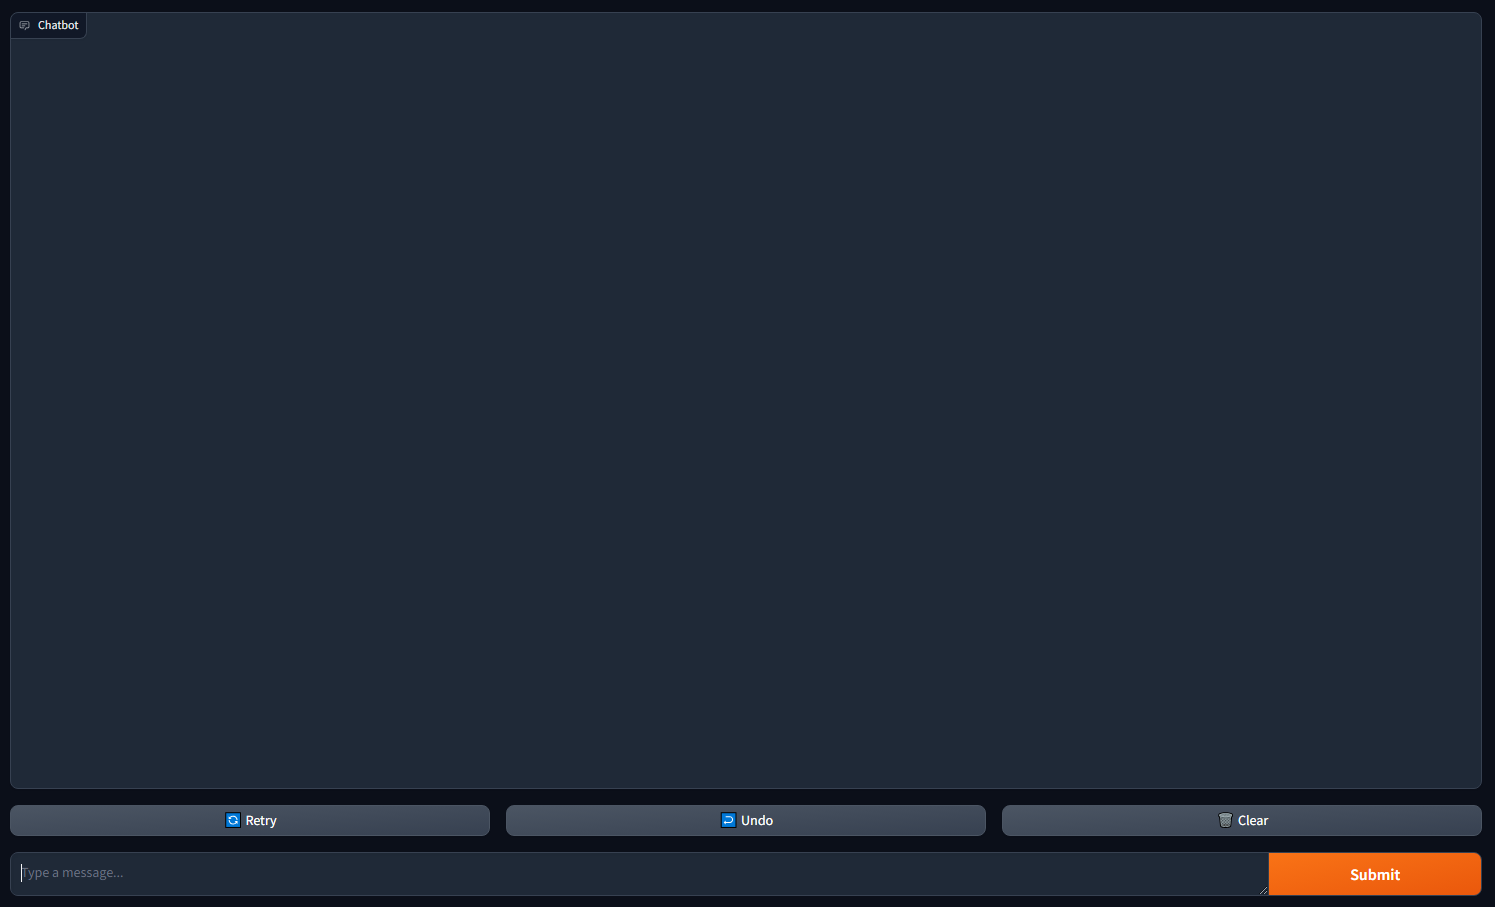
\includegraphics[width=1\textwidth]{img/guivacia.png}
    \caption{Interfaz gráfica de usuario}
    \label{fig:guivacia}
\end{figure}

\begin{figure}[h!]
    \centering
    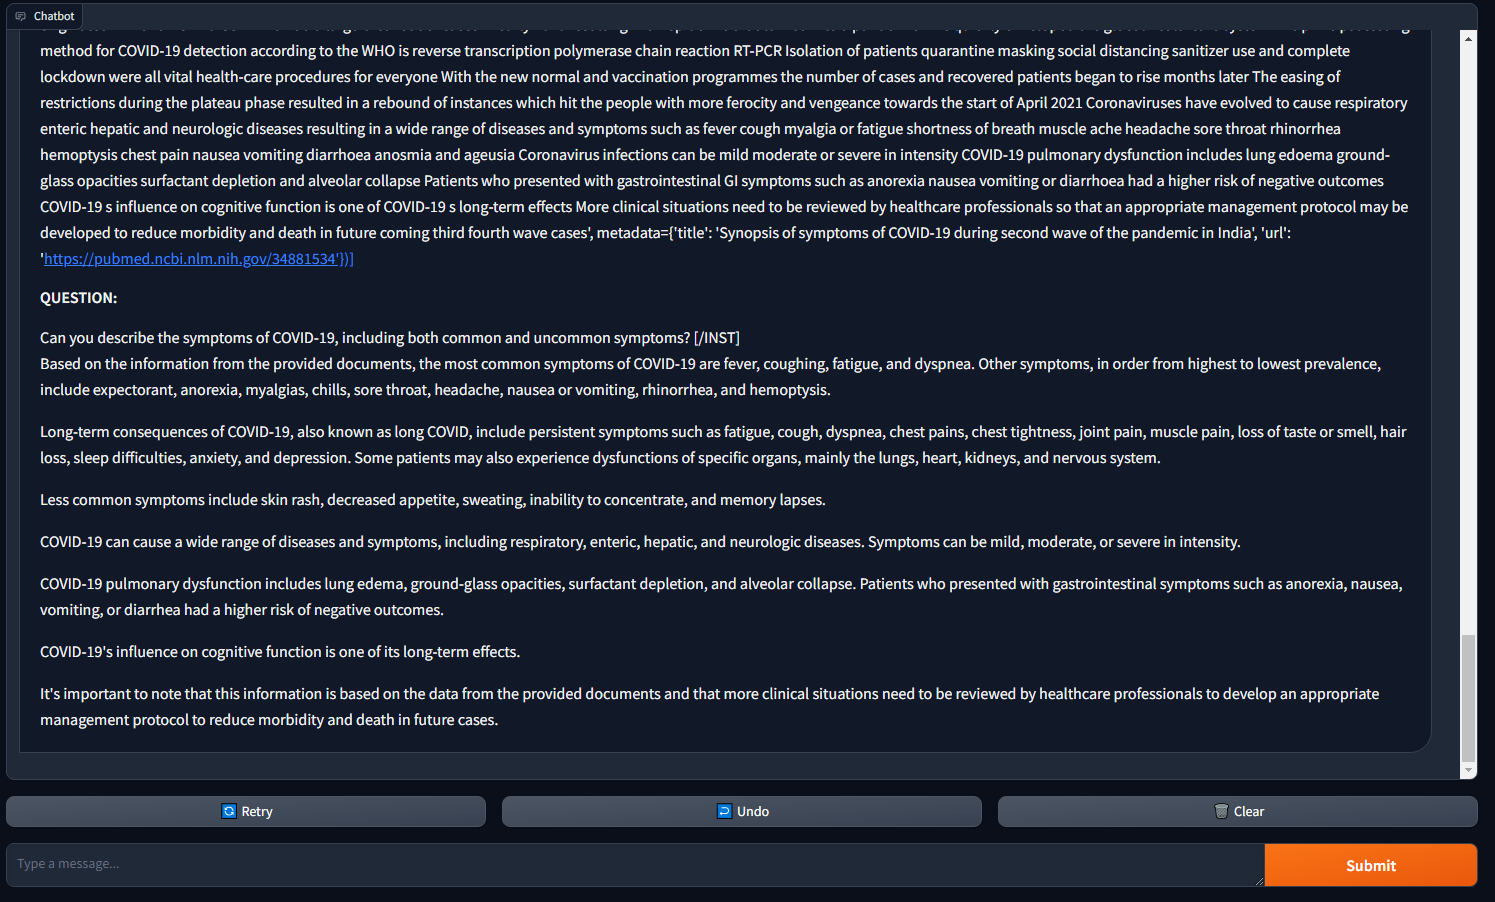
\includegraphics[width=1\textwidth]{img/guirellena.png}
    \caption{Interfaz gráfica de usuario tras una ejecución}
    \label{fig:guirellena}
\end{figure}

\FloatBarrier

\subsection{Salidas del programa}

En el anexo G se ha realizado una validación exhaustiva de diferentes salidas del programa, sin embargo en esta sección se observarán ejemplos distintos de las distintas posibles salidas.

\subsubsection{Salida sin retrieval}

En este ejemplo se propone un prompt que no tiene nada que ver con el tema en el que el programa está especializado, es decir, Covid-19. Se puede observar como no devuelve ningún abstract (el apartado de contexto está vacío, sólo se encuentra un []) ya que no hay ninguno en la base de datos vectorizada que sobrepase el threshold impuesto en la parametrización del retriever.

Prompt: What's the sun's mass?

Contexto: []

Salida: [INST] Instruction: You are an expert in microbiology. Please answer the question based ONLY on your knowledge of abstracts from a series of articles in this prompt don't use information of any other kind, if there were not any articles passed in this prompt just indicate that:
[]

QUESTION:
What's the sun's mass? [/INST]
I'm an expert in microbiology and I don't have the ability to directly answer questions about the mass of the sun based solely on the information from the abstracts provided in this prompt. The abstracts do not contain any information about the mass of the sun.

\subsubsection{Salida con retrieval específico}

En este caso se le hará una pregunta muy específica de la que hay pocos artículos que hablen, el retrieval será escueto ya que se prefiere recuperar poca información a recuperar bastante información que no tiene que ver con el tema ya que, en el ámbito biomédico, puede tener consecuencias fatales.

Prompt: What is the state of Covid in Spain?

Contexto: [INST] Instruction: You are an expert in microbiology. Please answer the question based ONLY on your knowledge of abstracts from a series of articles in this prompt don't use information of any other kind, if there were not any articles passed in this prompt just indicate that:
[Document(page\_content='OBJECTIVE The Spanish health system is made up of seventeen regional health systems Through the official reporting systems some inconsistencies and differences in case fatality rates between Autonomous Communities CC AA have been observed Therefore the objective of this paper is to compare COVID-19 case fatality rates across the Spanish CC AA MATERIAL AND METHODS Observational descriptive study The COVID-19 case fatality rate CFR was estimated according to the official records CFR-PCR the daily mortality monitory system MoMo record CFR-Mo and the seroprevalence study ENE-COVID-19 Estudio Nacional de sero Epidemiologia Covid-19 according to sex age group and CC AA between March and June 2020 The main objective is to detect whether there are any differences in CFR between Spanish Regions using two different register systems i e the official register of the Ministry of Health and the MoMo RESULTS Overall the CFR-Mo was higher than the CFR-PCR 1 59 vs 0 98 The differences in case fatality rate between both methods were significantly higher in Castilla La Mancha Castilla y Leon Cataluna and Madrid The difference between both methods was higher in persons over 74 years of age CFR-PCR 7 5 vs 13 0 for the CFR-Mo but without statistical significance There was no correlation of the estimated prevalence of infection with CFR-PCR but there was with CFR-Mo R2 0 33 Andalucia presented a SCFR below 1 with both methods and Asturias had a SCFR higher than 1 Cataluna and Castilla La Mancha presented a SCFR greater than 1 in any scenario of SARS-CoV-2 infection calculated with SCFR-Mo CONCLUSIONS The PCR case fatality rate underestimates the case fatality rate of the SARS-CoV- 2 virus pandemic It is therefore preferable to consider the MoMo case fatality rate Significant differences have been observed in the information and registration systems and in the severity of the pandemic between the Spanish CC AA Although the infection prevalence correlates with case fatality rate other factors such as age comorbidities and the policies adopted to address the pandemic can explain the differences observed between CC AA', metadata={'title': 'Analysis of case fatality rate of SARS-CoV-2 infection in the Spanish Autonomous Communities between March and May 2020', 'url': 'https://pubmed.ncbi.nlm.nih.gov/34860848'}), Document(page\_content='Measuring mortality has been a challenge during the COVID-19 pandemic Here we compared the results from the Spanish daily mortality surveillance system MoMo of excess mortality estimates using a time series analysis with those obtained for the confirmed COVID-19 deaths reported to the National Epidemiological Surveillance Network RENAVE The excess mortality estimated at the beginning of March 2020 was much greater than what has been observed in previous years and clustered in a very short time The cumulated excess mortality increased with age In the first epidemic wave the excess mortality estimated by MoMo was 1 5 times higher than the confirmed COVID-19 deaths reported to RENAVE but both estimates were similar in the following pandemic waves Estimated excess mortality and confirmed COVID-19 mortality rates were geographically distributed in a very heterogeneous way The greatest increase in mortality that has taken place in Spain in recent years was detected early by MoMo coinciding with the spread of the COVID-19 pandemic MoMo is able to identify risk situations for public health in a timely manner relying on mortality in general as an indirect indicator of various important public health problems', metadata={'title': 'The Impact of COVID-19 on Mortality in Spain Monitoring Excess Mortality MoMo and the Surveillance of Confirmed COVID-19 Deaths', 'url': 'https://pubmed.ncbi.nlm.nih.gov/34960692'})]

Salida:

QUESTION:
What is the state of Covid in Spain? [/INST]
Based on the provided abstracts, it appears that there have been inconsistencies and differences in case fatality rates (CFR) of COVID-19 between various Autonomous Communities (CC AA) in Spain. An observational descriptive study was conducted to compare CFR across Spanish regions using two different register systems: the official register of the Ministry of Health and the MoMo daily mortality monitoring system.

The study found that the CFR from the MoMo system was higher than the CFR from the official register (1.59 vs 0.98). Significant differences in CFR were observed between Castilla La Mancha, Castilla y Leon, Cataluna, and Madrid using both methods. The difference between methods was higher in persons over 74 years of age. There was no correlation of infection prevalence with CFR from the official register, but there was a correlation with CFR from the MoMo system. Andalucia presented a case fatality rate below 1 with both methods, while Asturias had a case fatality rate higher than 1. Cataluna and Castilla La Mancha presented a case fatality rate greater than 1 in any scenario of SARS-CoV-2 infection calculated with the MoMo system.

Another study compared the results from the Spanish daily mortality surveillance system (MoMo) of excess mortality estimates with those obtained for confirmed COVID-19 deaths reported to the National Epidemiological Surveillance Network (RENAVE). The study found that the excess mortality estimated at the beginning of March 2020 was much greater than what has been observed in previous years and clustered in a very short time. The cumulated excess mortality increased with age. In the first epidemic wave, the excess mortality estimated by MoMo was 1.5 times higher than the confirmed COVID-19 deaths reported to RENAVE, but both estimates were similar in the following pandemic waves. The greatest increase in mortality that has taken place in Spain in recent years was detected early by MoMo, coinciding with the spread of the COVID-19 pandemic. MoMo is able to identify risk situations for public health in a timely manner, relying on mortality in general as an indirect indicator of various important public health problems.

In summary, the studies suggest that there are significant differences in CFR between Spanish regions and that the MoMo system may provide a more accurate estimate of CFR during the COVID-19 pandemic. Excess mortality estimates from MoMo have identified risk situations for public health in a timely manner. However, it is important to note that other factors such as age, comorbidities, and policies adopted to address the pandemic can also explain the differences observed between CC AA.


\subsubsection{Salida con retrieval específico}

Al igual que en el anterior caso se hará una cuestión sobre la que será posible recuperar contexto, en este caso se hará una petición general y los abstrracts que recuperará serán los más relevantes de entre varios recuperados que superan el threshold.

Prompt: Name the most common symptoms of Covid-19, present the data in a list

Context: [Document(page\_content='BACKGROUND The new coronavirus disease COVID-19 carries a high risk of infection and has spread rapidly around the world However there are limited data about the clinical symptoms globally The purpose of this systematic review and meta-analysis is to identify the prevalence of the clinical symptoms of patient with COVID-19 METHODS A systematic review and meta-analysis were carried out The following databases were searched PubMed CINAHL MEDLINE EMBASE PsycINFO medRxiv and Google Scholar from December 1st 2019 to January 1st 2021 Prevalence rates were pooled with meta-analysis using a random-effects model Heterogeneity was tested using I-squared I 2 statistics RESULTS A total of 215 studies involving 132 647 COVID-19 patients met the inclusion criteria The pooled prevalence of the four most common symptoms were fever 76 2 n 214 95 CI 73 9-78 5 coughing 60 4 n 215 95 CI 58 6-62 1 fatigue 33 6 n 175 95 CI 31 2-36 1 and dyspnea 26 2 n 195 95 CI 24 1-28 5 Other symptoms from highest to lowest in terms of prevalence include expectorant 22 2 anorexia 21 6 myalgias 17 5 chills 15 sore throat 14 1 headache 11 7 nausea or vomiting 8 7 rhinorrhea 8 2 and hemoptysis 3 3 In subgroup analyses by continent it was found that four symptoms have a slight prevalence variation-fever coughing fatigue and diarrhea CONCLUSION This meta-analysis found the most prevalent symptoms of COVID-19 patients were fever coughing fatigue and dyspnea This knowledge might be beneficial for the effective treatment and control of the COVID-19 outbreak Additional studies are required to distinguish between symptoms during and after in patients with COVID-19', metadata={'title': 'Clinical Features of COVID-19 Patients in the First Year of Pandemic A Systematic Review and Meta-Analysis', 'url': 'https://pubmed.ncbi.nlm.nih.gov/34866409'}), Document(page\_content='COVID-19 was caused by the original coronavirus severe acute respiratory syndrome associated coronavirus-2 SARS CoV2 which originated in Wuhan China COVID-19 had a large breakout of cases in early 2020 resulting in an epidemic that turned into a pandemic This quickly enveloped the global healthcare system The principal testing method for COVID-19 detection according to the WHO is reverse transcription polymerase chain reaction RT-PCR Isolation of patients quarantine masking social distancing sanitizer use and complete lockdown were all vital health-care procedures for everyone With the new normal and vaccination programmes the number of cases and recovered patients began to rise months later The easing of restrictions during the plateau phase resulted in a rebound of instances which hit the people with more ferocity and vengeance towards the start of April 2021 Coronaviruses have evolved to cause respiratory enteric hepatic and neurologic diseases resulting in a wide range of diseases and symptoms such as fever cough myalgia or fatigue shortness of breath muscle ache headache sore throat rhinorrhea hemoptysis chest pain nausea vomiting diarrhoea anosmia and ageusia Coronavirus infections can be mild moderate or severe in intensity COVID-19 pulmonary dysfunction includes lung edoema ground-glass opacities surfactant depletion and alveolar collapse Patients who presented with gastrointestinal GI symptoms such as anorexia nausea vomiting or diarrhoea had a higher risk of negative outcomes COVID-19 s influence on cognitive function is one of COVID-19 s long-term effects More clinical situations need to be reviewed by healthcare professionals so that an appropriate management protocol may be developed to reduce morbidity and death in future coming third fourth wave cases', metadata={'title': 'Synopsis of symptoms of COVID-19 during second wave of the pandemic in India', 'url': 'https://pubmed.ncbi.nlm.nih.gov/34881534'}), Document(page\_content='Many patients who had coronavirus disease 2019 COVID-19 had at least one symptom that persisted after recovery from the acute phase Our purpose was to review the empirical evidence on symptom prevalence complications and management of patients with long COVID We systematically reviewed the literature on the clinical manifestations of long COVID-19 defined by the persistence of symptoms beyond the acute phase of infection Bibliographic searches in PubMed and Google Scholar were conducted to retrieve relevant studies on confirmed patients with long COVID that were published prior to August 30 2021 The most common persistent symptoms were fatigue cough dyspnea chest pains chest tightness joint pain muscle pain loss of taste or smell hair loss sleep difficulties anxiety and depression Some of the less common persistent symptoms were skin rash decreased appetite sweating inability to concentrate and memory lapses In addition to these general symptoms some patients experienced dysfunctions of specific organs mainly the lungs heart kidneys and nervous system A comprehensive understanding of the persistent clinical manifestations of COVID-19 can improve and facilitate patient management and referrals Prompt rehabilitative care and targeted interventions of these patients may improve their recovery from physical immune and mental health symptoms', metadata={'title': 'Persistence of Symptoms After Discharge of Patients Hospitalized Due to COVID-19', 'url': 'https://pubmed.ncbi.nlm.nih.gov/34881263'}), Document(page\_content='Background The SARS-CoV-2 disease called COVID-19 emerged in China has acquired pandemic dimensions According to the WHO situational report of March 15 2021 the global fatality rate is 2 2 in Mexico around 194 944 deaths have been confirmed by COVID-19 Studies in China identified that patients with severe COVID-19 when compared with those who had non-severe COVID-19 presented more severe neurological manifestations Objective To determine the frequency of neurological symptoms and manifestations in patients with severe COVID-19 in a tertiary care center Material and methods A cross-sectional observational and analytical study was carried out at the Hospital de Especialidades del Centro Medico Nacional Siglo XXI in patients hospitalized with severe COVID-19 Results 183 cases were analyzed of which 130 were men 71 The median age was 55 years IQR 44-65 The neurological symptoms were headache anosmia and dysgeusia Neurological manifestations occurred in 27 patients 16 the most frequent was ischemic-type cerebrovascular disease CVD in 12 44 in patients older than 76 5 years vs 54 years p 0 000 with history of cardiovascular disease Conclusions The most frequent neurological symptoms were headache anosmia and dysgeusia The most frequent neurological manifestation was ischemic CVD that appeared in older patients with severe COVID-19 with a history of cardiovascular disease', metadata={'title': 'Neurological manifestations in patients with severe COVID-19 in a tertiary care center', 'url': 'https://pubmed.ncbi.nlm.nih.gov/34910416'})]

Salida: Name the most common Symptoms of Covid-19, present the data in a list [/INST]

1. Fever: Prevalence rate = 76.2\% (CI: 73.9-78.5\%)
2. Coughing: Prevalence rate = 60.4\% (CI: 58.6-62.2\%)
3. Fatigue: Prevalence rate = 33.6\% (CI: 31.2-36.1\%)
4. Dyspnea: Prevalence rate = 26.2\% (CI: 24.1-28.3\%)
These symptoms were identified from the systematic review and meta-analysis of 132,647 COVID-19 patients across various studies.

\section{Discusión.}

En esta capitulo se encontrará una discusión y análisis de los resultados obtenidos, no obstante primero a forma de introducción resulta interesante recordar los objetivos.

\begin{enumerate}

    \item Cómo requisitos software se planteaba el desarrollo de una aplicación de chatbot que generase respuestas altamente especializadas con una interfaz amigable e intuitiva.
    
    \item Los objetivos de carácter técnico recalcaban la calidad que tenía que tener el proyecto, aportando respuestas de gran calidad tanto científica como de redacción.
    
    \item Finalmente los objetivos de aprendizaje hacían hincapié en el estudio de los modelos grandes de lenguaje (LLMs), su especialización en información recopilada mediante el proceso de RAG y la aplicación de todo ello al ámbito de la investigación biomédica.
    
\end{enumerate}

\subsection{Discusión de la aplicación}

La interfaz presentada resulta altamente intuitiva y no se requiere ningún conocimiento previo en informática para su correcto uso, con solo tres botones opcionales y un mecanismo básico de pregunta-respuesta se considera cumplido el objetivo planteado en cuanto a la intuitividad.

\subsection{Discusión de las salidas}

Las salidas presentadas tanto en este capítulo como en el anexo experimental presentan una alta calidad científica y de redacción, se ha demostrado que el retrieval sólo se realiza en el caso de que tenga relevancia con la petición, en caso contrario se informa de ello y que la información recuperada está presente en los abstracts. También se devuelve la url relativa al paper completo del abstract recuperado, esto es un éxito ya que permite a los usuarios acceder a toda la información completa y permite a la aplicación tomar un carácter proactivo, proporcionando no únicamente una respuesta sino que ayuda al científico a ampliar la información. Los datos sobre los que se realiza todo el proceso de RAG son datos validados, contrastados y públicos, se pueden consultar en cualquier momento en PubMed. 